\documentclass[style=upen, size=14pt]{powerdot}
\usepackage{natbib}
\usepackage{bibentry}
\usepackage{mathtools}
\definecolor{arany}{RGB}{255,242,0}
\hypersetup{backref=page}
\hypersetup{
    colorlinks=true,
    linkcolor=cyan,
    citecolor=cyan,
    filecolor=magenta,      
    urlcolor=cyan}
% \pdsetup{trans=Split}
\usepackage{graphicx}
\usepackage{amsmath}
\DeclareMathOperator*{\argmax}{argmax}
\DeclareMathOperator*{\argmin}{argmin}
\DeclareMathOperator*{\softmax}{softmax}
\DeclareMathOperator{\sign}{sign}
\usepackage{amssymb}
\usepackage{stmaryrd}
\usepackage[latin2]{inputenc}
%\usepackage[magyar]{babel}
%\usepackage{euler}
\usepackage{tikz}
\usetikzlibrary{matrix}
%\usepackage{tikz-qtree}
%\usepackage{tikz-dependency}
%\usepackage{linguex}
\usepackage{amsthm}
\usepackage{amsmath}
%\tikzset{every tree node/.style={align=center,anchor=north}}
%\usepackage{tabularx}
%\usepackage{threeparttable}
%\usepackage{color}
%\selectlanguage{english}
%\frenchspacing
\usepackage{algpseudocode}
\usepackage{algorithm}
\newcommand\varlist{,\makebox[1em][c]{.\hfil.\hfil.},}
\newcommand{\nd}{\noindent}
\newcommand{\Val}{\mathop{\mathit{Val}}}
\newcommand{\gold}{\color{arany}}
%\usepackage{tikz}
%\usepackage{tikz-qtree}
%\newcommand{\qed}{\hfill\mbox{\raggedright \rule{.1in}{.1in}}}
\def\es{\mathbin\land}
\theoremstyle{definition}
\newtheorem*{definition}{Definition}
\newtheorem{axioma}{Axiom}
\newtheorem{tetel}{Theorem}
\newtheorem{prop}{Proposition}
\newtheorem{lemma}{Lemma}
\begin{document}

\title{Natural Language Processing\\~~\\Lecture 9\\RNNs and language modeling}
% \author{}

\date{2021}
\maketitle


\section[toc=Introduction]{Introduction}

\begin{slide}[toc=NN-based LMs]{Language modeling with NNs}
  As we have seen, feedforward NN language models with word embeddings already
  performed better than traditional $n$-gram models, e.g.,
  \cite{bengio2003neural}:
  \begin{center}
    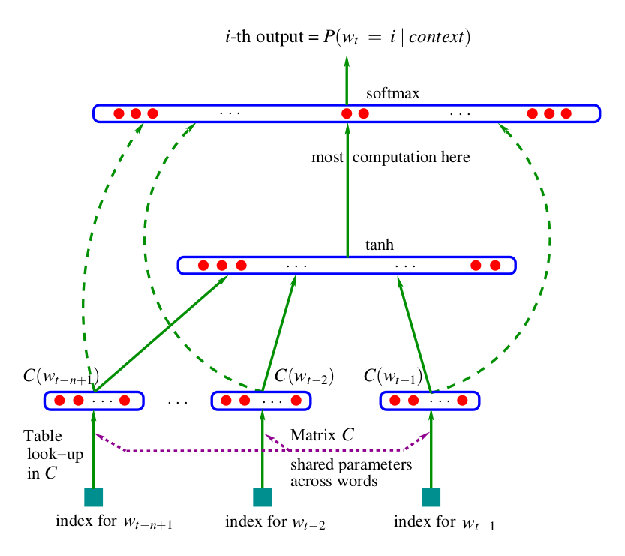
\includegraphics[width=0.6\textwidth]{figures/neural_lm.eps}
  \end{center}
\end{slide}

\begin{slide}[toc=]{Language modeling with NNs cont.}
  \cite{bengio2003neural} reports 24\% improvement in perplexity compared to the
  best $n$-gram model.\bigskip
  
  But these models still share an important limitation of $n$-gram models: the
  continuation predictions are based on a \emph{fixed size context window},
  without any information on earlier history:
  $$
  \hat P(w_{t}~|~w_0,\dots,w_{t-1}) = \phi(w_{t-k},\dots, w_{t-1}),
  $$
  where $\phi(\cdot)$ is a function computed by a feedforward neural network.
\end{slide}

\begin{slide}[toc=RNNs]{Recurrent Neural Networks (RNNs)}
  \emph{Recurrent neural networks}, in contrast, are not limited to fixed-length
  input sequences, and can form, at least in theory, useful internal
  representations of \emph{arbitrary long} histories. They can process
  sequential input step-by-step and keep an internal state which can be updated
  at each step:
  \begin{center}
    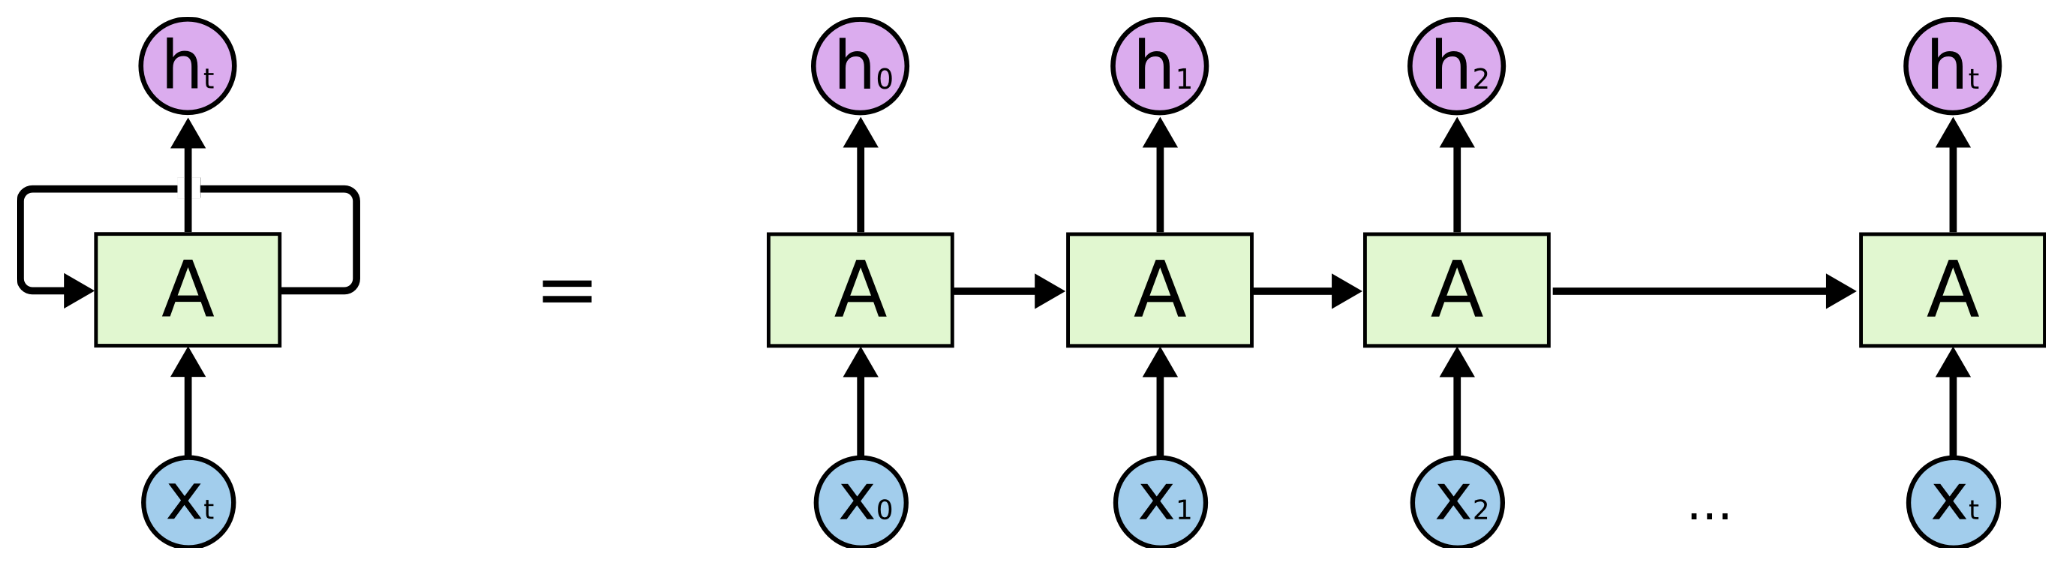
\includegraphics[width=1\textwidth]{figures/RNN-unrolled.eps}
    \footnotesize{If not otherwise indicated, figures in this and the next
      section are from \cite{olah2015understanding}.}
  \end{center}
\end{slide}

\begin{slide}[toc=]{Recurrent Neural Networks cont.}
  RNNs can have rather simple internal structure, e.g., the once widely used
  Elman network\footnote{\cite{elman1990finding}.} has a structure
  \begin{center}
    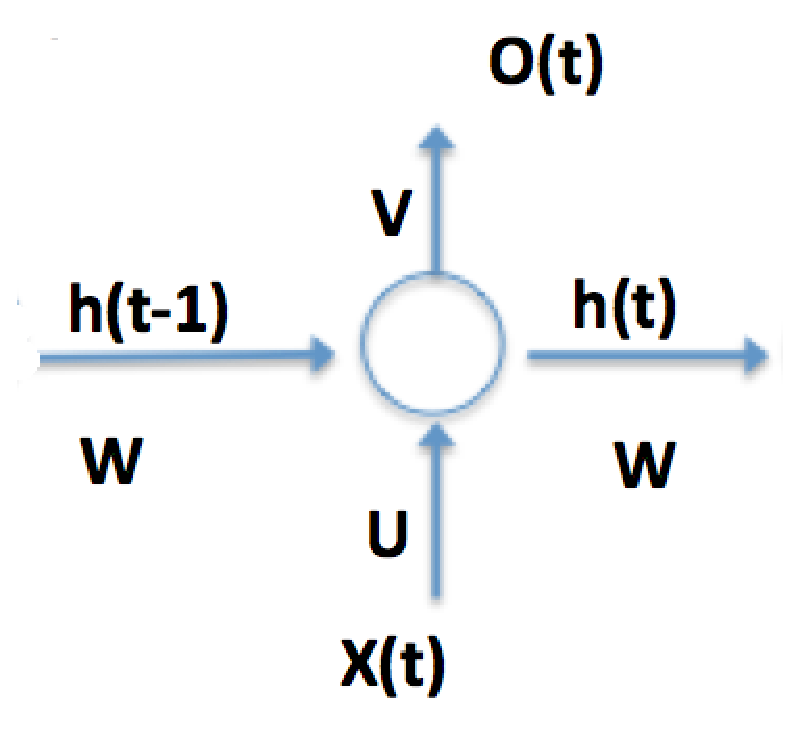
\includegraphics[width=0.3\textwidth]{figures/elman.eps}
  \end{center}
  $$
  h_t = a_h(U x_t + W h_{t-1} + b_h ),
  $$
  $$
  o_t = a_o(Vh_{t} + b_o ).
  $$
\end{slide}

\begin{slide}[toc=BPTT]{Backpropagation through time}
  The standard optimization method for RNNs is \emph{backpropagation through
    time} (BPTT), which is backpropagation applied to the time-unfolded network:
  \begin{center}
    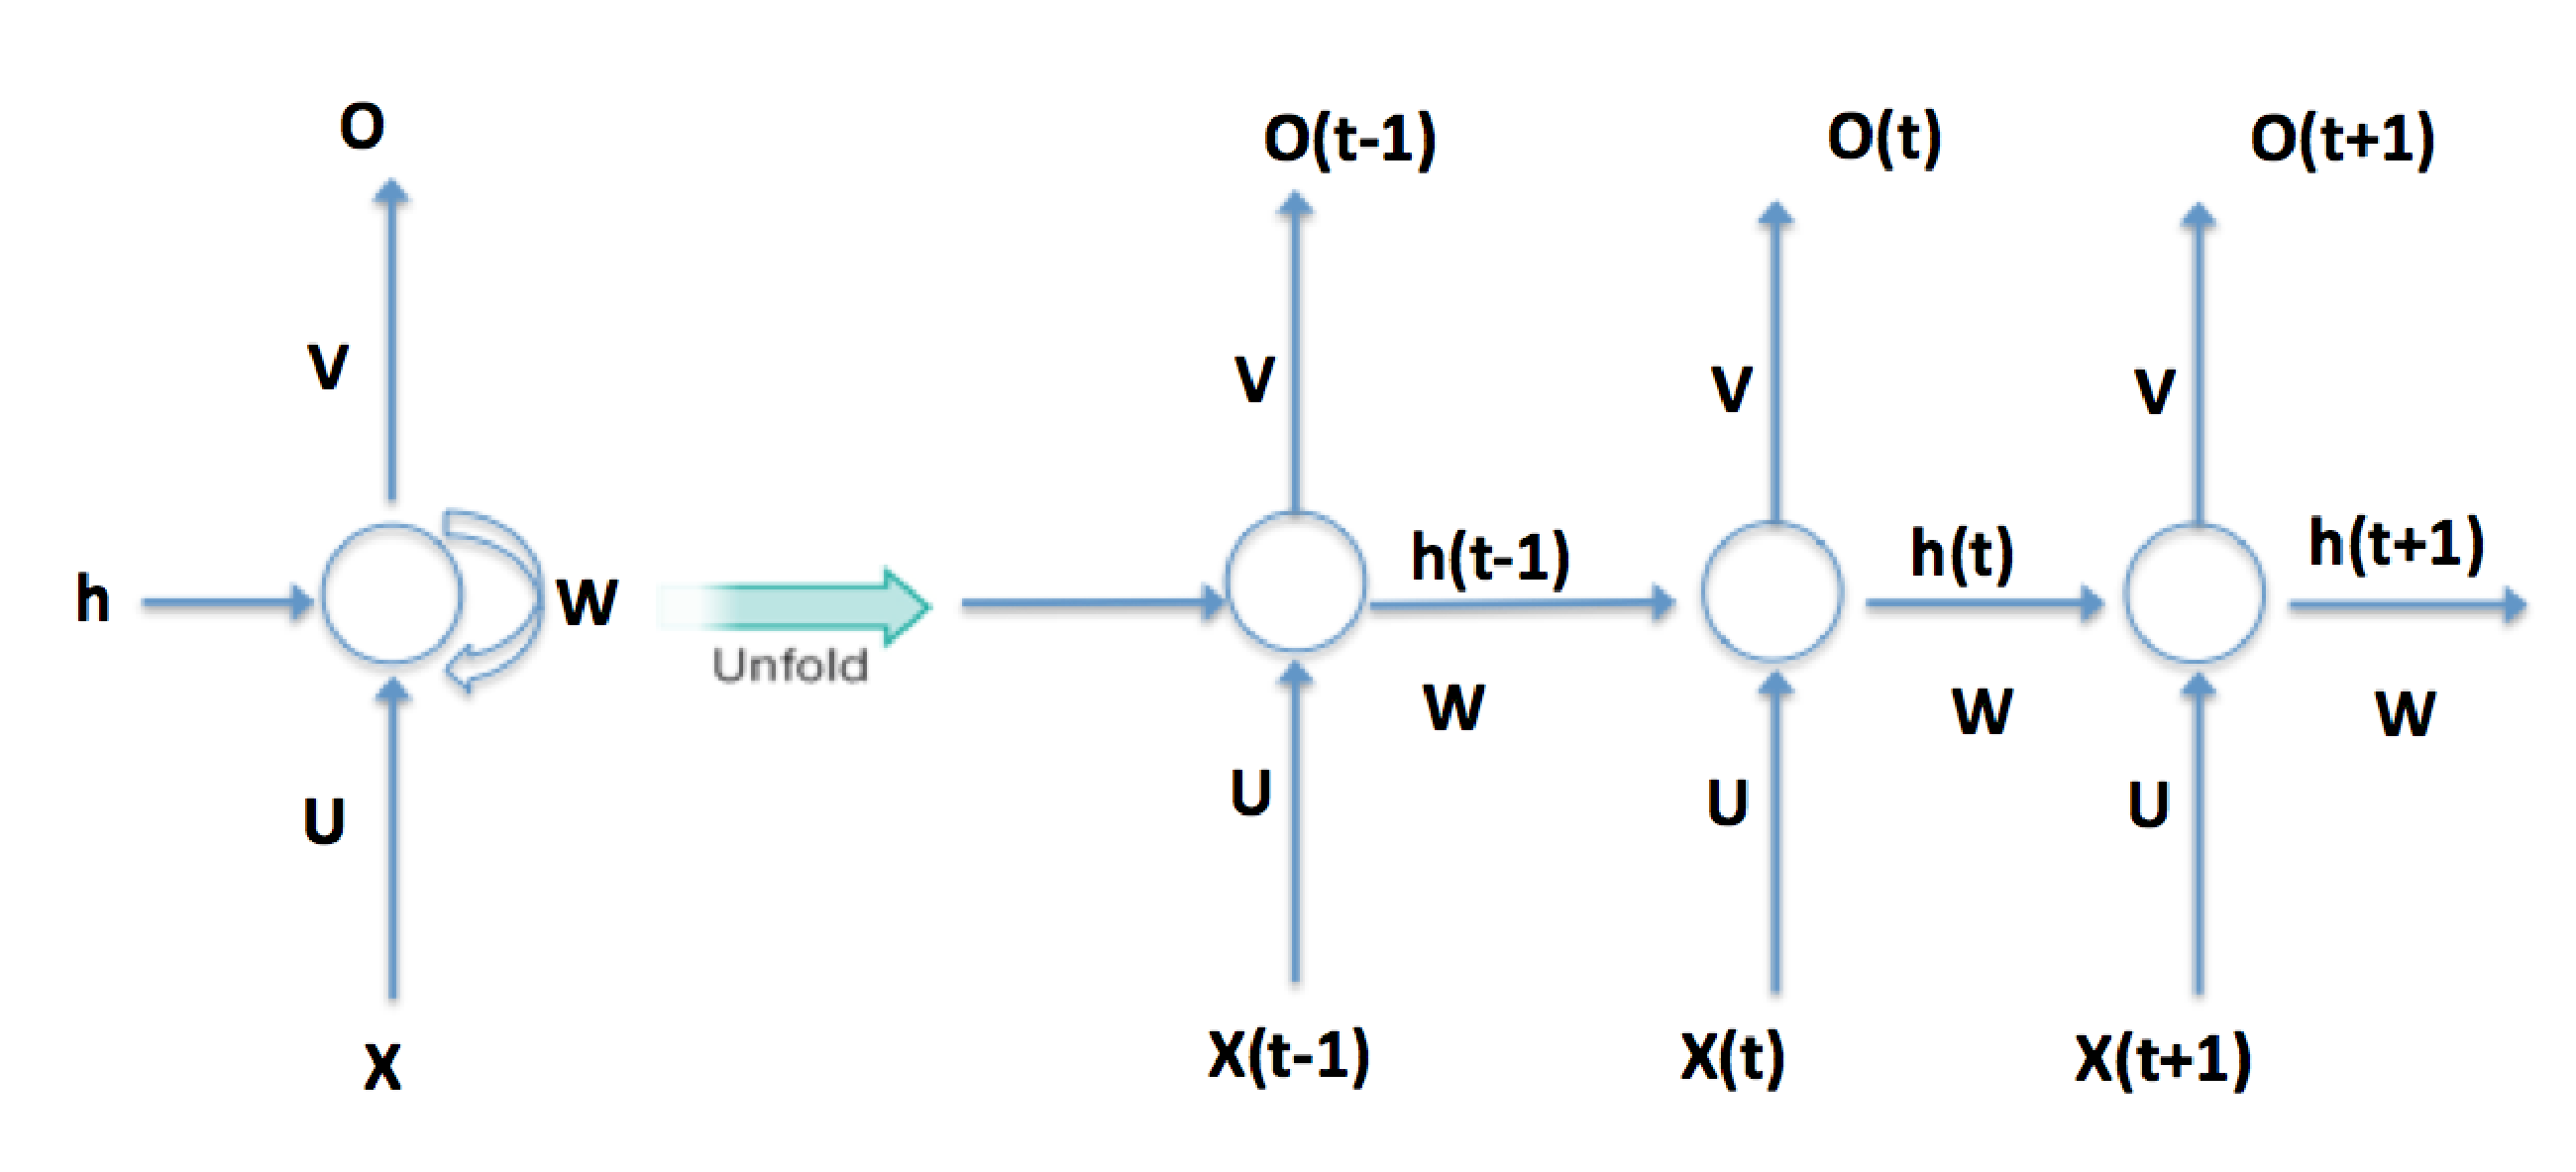
\includegraphics[width=0.95\textwidth]{figures/rnn_unrolling.eps}
  \end{center}
\end{slide}

\begin{slide}[toc=]{Backpropagation through time cont.}
  Since the depth of an unrolled RNN grows linearly with the number of time
  steps through which it is unrolled, it is often unfeasible to do
  backpropagation through all time steps until the first one. \bigskip

  In these cases, unrolling and backpropagation of error is only done for a
  certain number of time steps -- \emph{\gold backpropagation is truncated}. In practice,
  most neural network frameworks implement truncated backpropagation.
\end{slide}

\begin{slide}[toc=Challenges]{RNN training challenges}
  Training RNNs poses significant challenges:
  \begin{itemize}
  \item An RNN unrolled through several timesteps is behaving like a deep
    feedforward network with respect to backpropagation, so both \emph{\gold
      vanishing} and \emph{\gold exploding gradients} can be a problem,
    exacerbated by the fact that the exact same layers are repeated.
  \item Vanishing gradients, in particular, mean that the RNN does not learn
    \emph{\gold long-term dependencies}, which, in theory, should be its
    strength.
  \end{itemize}
\end{slide}

\section[toc=LSTMs]{Long Short-Term Memory Networks}

\begin{slide}[toc=LSTM]{Long Short-Term Memory (LSTM)}
  \cite{hochreiter1997long} introduced an elaborate gated topology to endow RNNs
  with long-term memory and solve the vanishing/exploding gradients problem.
  \begin{center}
    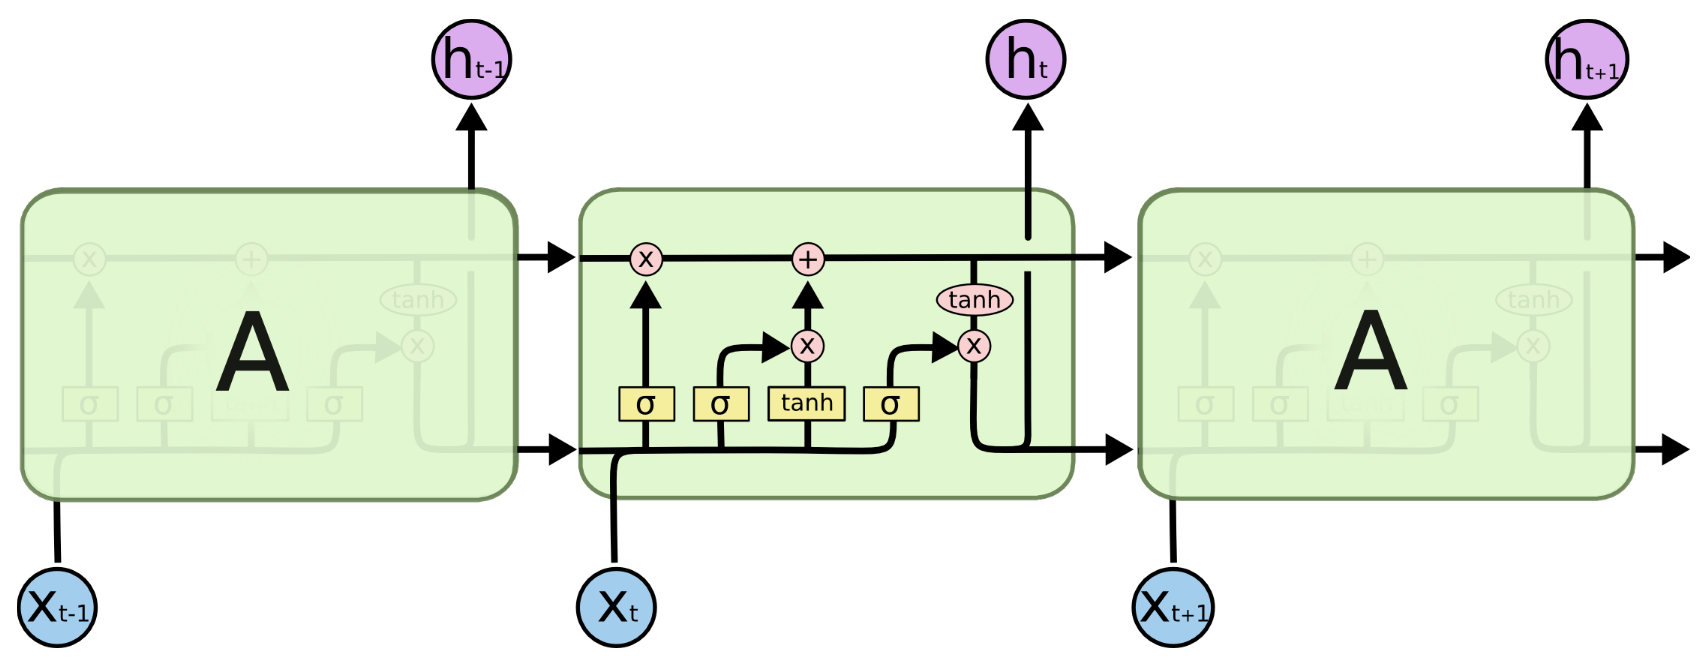
\includegraphics[width=1\textwidth]{figures/LSTM3-chain.eps}
  \end{center}
\end{slide}

\begin{slide}{Cell state}
  The LSTM's cell state acts as an ``information conveyor belt'', on which
  information can travel across time steps.
  \begin{center}
    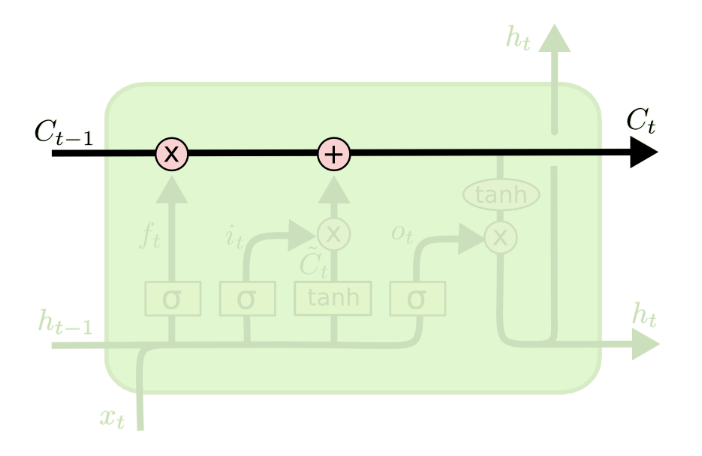
\includegraphics[width=0.65\textwidth]{figures/lstm_c_line.eps}
  \end{center}
\end{slide}

\begin{slide}{Forget gate}
  The forget gate calculates an $f_t\in (0,1)^d$ mask for removing information
  from the cell state:
  \begin{center}
    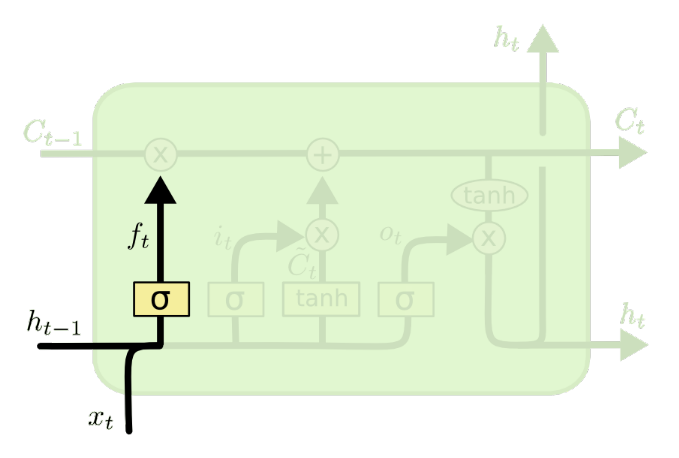
\includegraphics[width=0.65\textwidth]{figures/lstm_forget.eps}
  \end{center}
  $$
  f_t=\sigma(W_f[h_{t-1}, x_t] + b_f).
  $$
\end{slide}

\begin{slide}[toc=Input and update]{Input gate and update vector}
  An $i_t$ input mask and a $\tilde C_t$ update vector is calculated:
  \begin{center}
    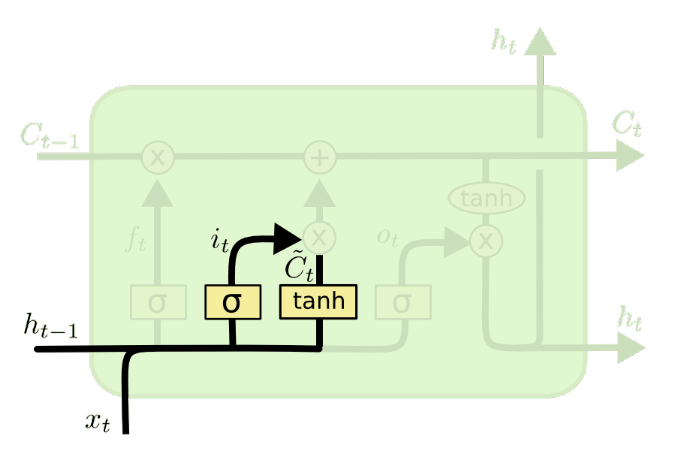
\includegraphics[width=0.65\textwidth]{figures/lstm_update.eps}
  \end{center}
  $$
  i_t=\sigma(W_i[h_{t-1}, x_t] + b_i),
  $$
  $$
  \tilde C_t = \tanh(W_C[h_{t-1}, x_t] + b_C).
  $$
\end{slide}

\begin{slide}[toc=New cell state]{Computing the new cell state}
  The new cell state can be computed using $f_t, i_t$ and
  $\tilde C_t$:
  \begin{center}
    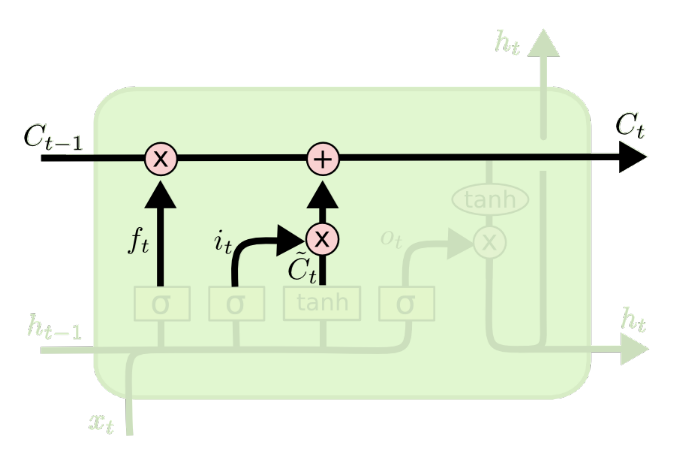
\includegraphics[width=0.65\textwidth]{figures/lstm_c.eps}
  \end{center}
  $$
  C_t = f_t \odot C_{t-1} + i_t \odot \tilde C_t.
  $$
\end{slide}

\begin{slide}[toc=Output]{Output}
  Finally, an output, $h_t$ is generated:
  \begin{center}
    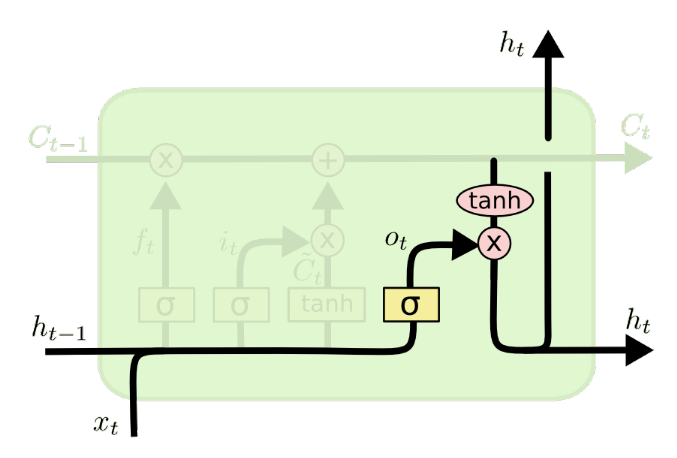
\includegraphics[width=0.65\textwidth]{figures/lstm_out.eps}
  \end{center}
  $$
  o_t = \sigma(W_o[h_{t-1}, x_t] + b_o),
  $$
  $$
  h_t = o_t \odot \tanh(C_t).
  $$
\end{slide}

\begin{slide}[toc=Advantages]{LSTM advantages}
  The gated LSTM architecture solves the problem of vanishing/exploding
  gradients by ensuring that the gradient can flow to distant time steps.\bigskip

  The fact that the updates are \emph{additive} means that gradients are not
  multiplied as in the Elman network's case, and the gates can acquire weights
  during training that allow the network to exhibit long-range dependencies
  between input and output values.
\end{slide}

\begin{slide}[toc=Peephole connections]{LSTM variants: Peephole connections}
  Peephole connections extend the LSTM architecture by giving access to the
  actual cell state to the gates:
  \begin{center}
    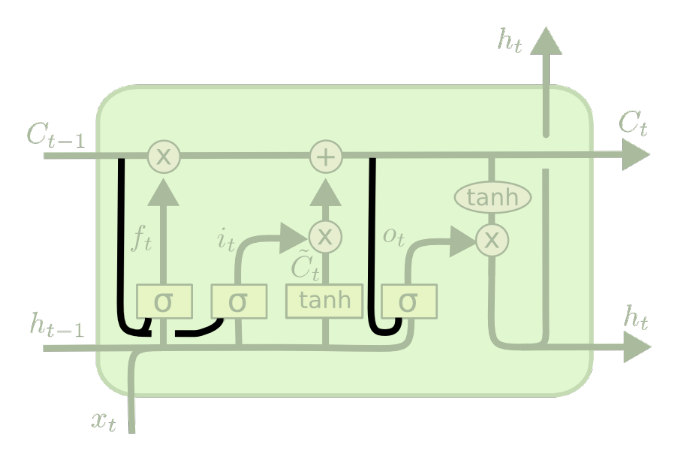
\includegraphics[width=0.65\textwidth]{figures/peepholes.eps}
  \end{center}
\end{slide}


\begin{slide}[toc=GRU]{LSTM variants: Gated Recurrent Unit (GRU)}
  GRU is a simplified LSTM variant, it gets rid of the separate cell
  state and merges the forget and input gates:
  \begin{center}
    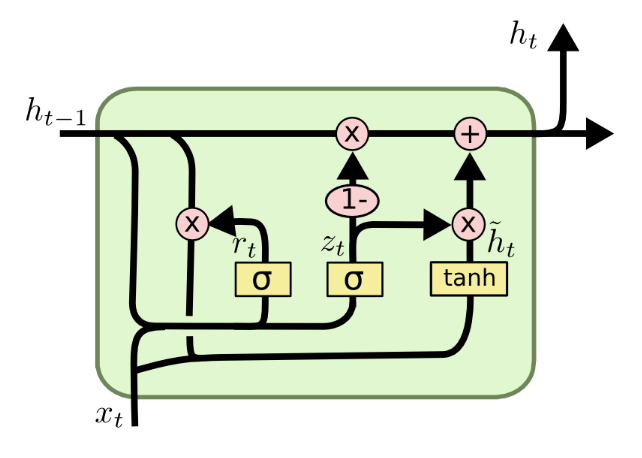
\includegraphics[width=0.65\textwidth]{figures/gru.eps}
  \end{center}
\end{slide}

\section[toc=LMs with RNNs]{Language modeling with RNNs}

\begin{slide}{Language modeling with RNNs}
  \begin{center}
    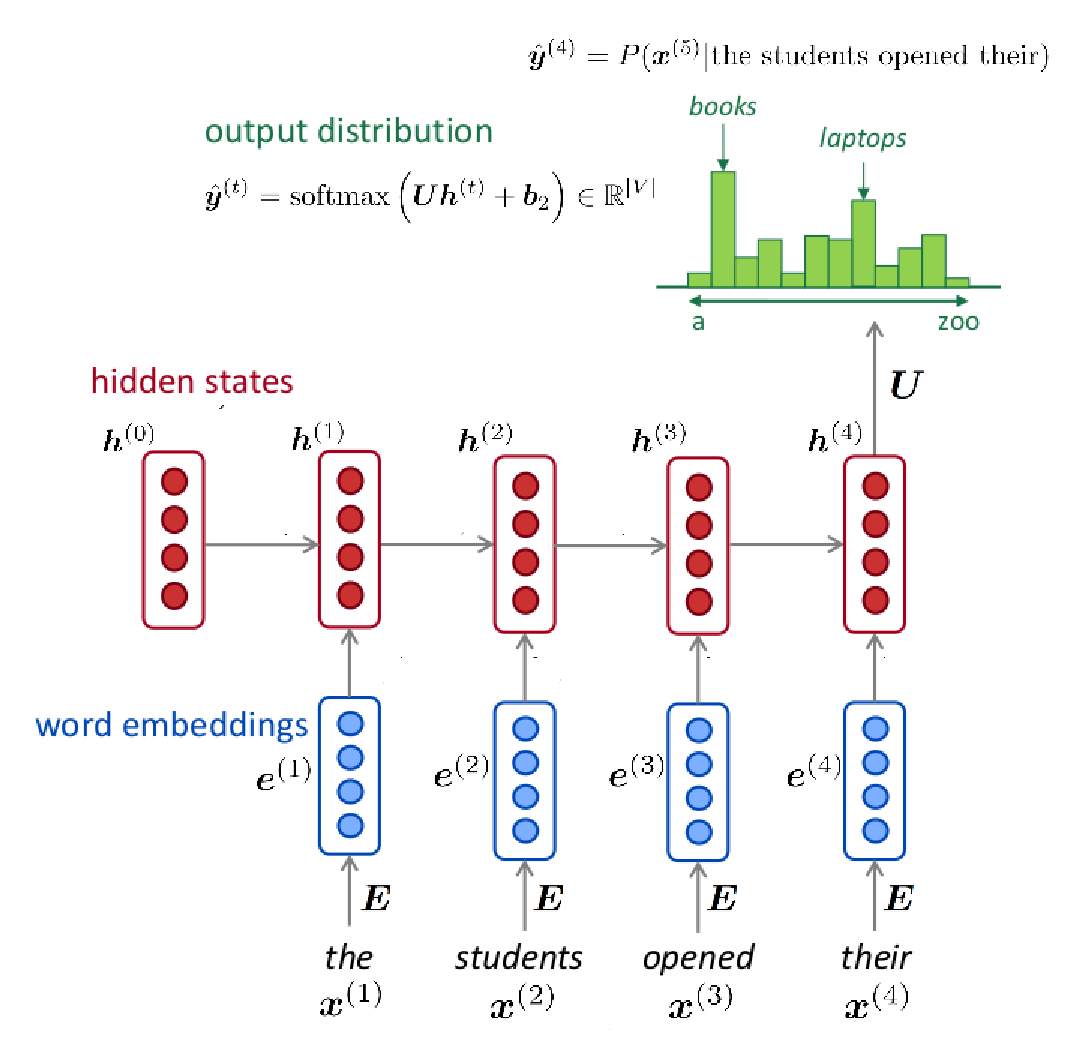
\includegraphics[width=0.7\textwidth]{figures/rnn_lm.eps}
  \end{center}
\end{slide}

\begin{slide}[toc=]{Language modeling with RNNs cont.}
  The most notable features of the model are
  \begin{itemize}
  \item previous words (``left context'') are processed step-by-step, one word
    at a time step;
  \item the first layer is a static word embedding;
  \item the $h_t$ RNN direct output (hidden state) gets transformed to a
    continuation probability distribution over the vocabulary by an affine
    transformation and the $\softmax$ nonlinearity.
  \end{itemize}
\end{slide}

\begin{slide}[toc=Sequence elements]{Sequence elements}
  Although traditionally RNN language models were word based, i.e., the sequence
  elements were words, there are two important alternatives:
  \begin{itemize}
  \item \emph{\gold character-level} language models treat characters as the
    sequence elements, and predict the next character based on the previous ones.
  \item \emph{\gold subword-level} language models are based on subword
    tokenization (e.g., BPE) and predict the next \emph{subword} in the
    vocabulary.
  \end{itemize}
  Both types of model can utilize corresponding -- character- and subword- --
  embeddings.
\end{slide}

\begin{slide}[toc=Training]{Training}
  RNN-based language models, as all parametric language models, are trained
  using the usual negative log-likelihood loss: if the training sequence is
  $\langle w_1,\dots, w_n \rangle$ and $\hat P_i$ is the model's output
  distribution for the $i$th continuation probability, then the loss is

  $$
  - \sum_{i=1}^n \log \hat P_i(w_i).
  $$
  But what should the \emph{input} of the RNN be at each time step during
  training? Should it come from the training data, or from the RNN's previous
  prediction?
\end{slide}

\begin{slide}[toc=]{Training cont.}
  RNN language models are typically trained using the training data as input.
  This is called \emph{\gold teacher forcing}.
  \begin{center}
    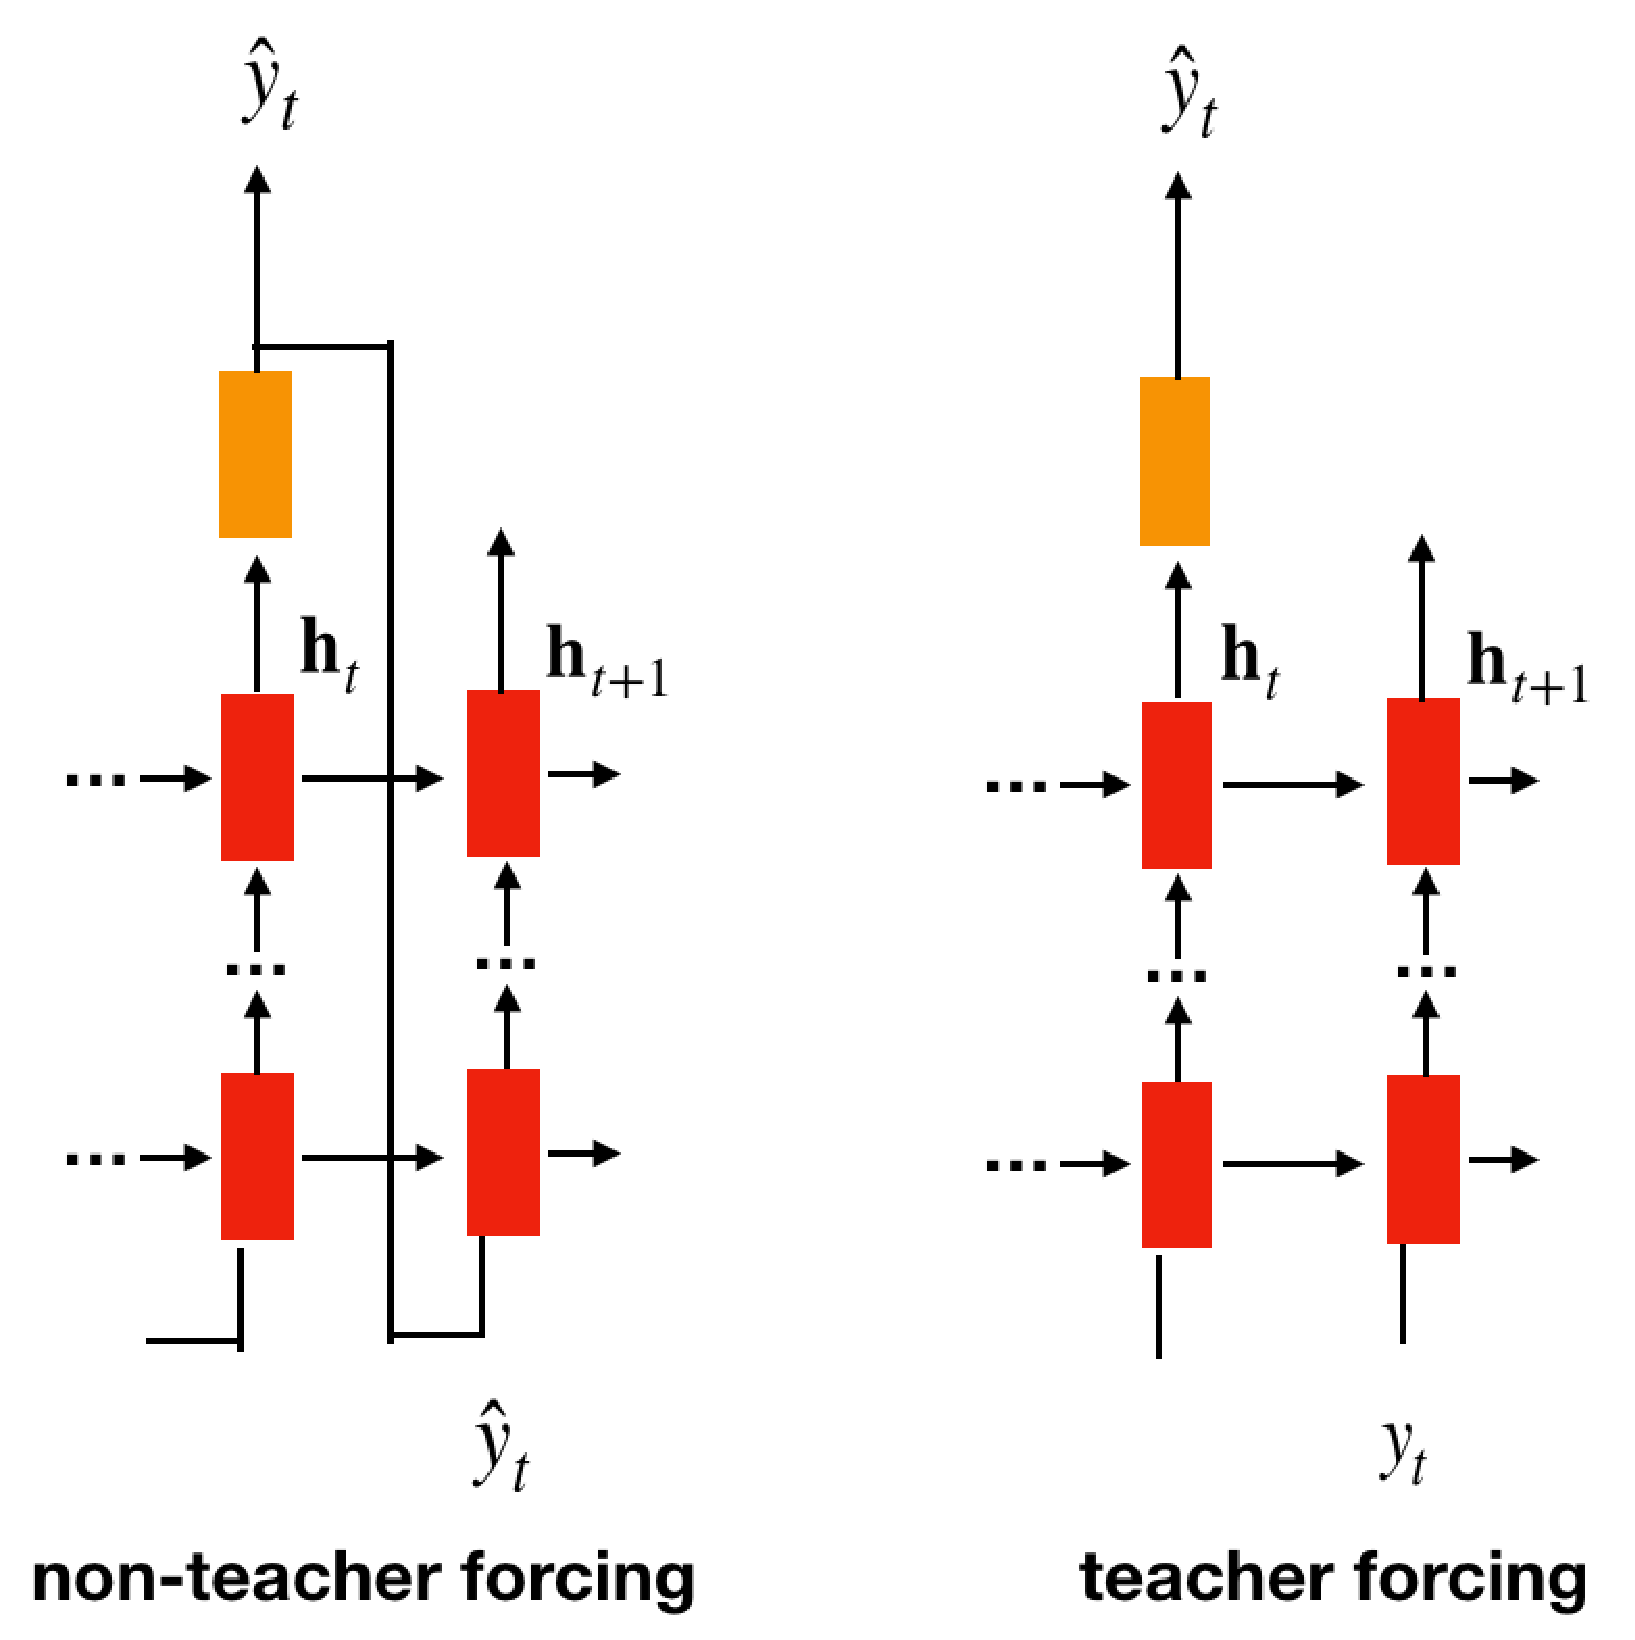
\includegraphics[width=0.55\textwidth]{figures/teacher_forcing.eps}
  \end{center}
\end{slide}

\begin{slide}[toc=Exposure bias]{Exposure bias}
  Although teacher forcing is by far the most used training method, it has a
  major problem, the phenomenon called \emph{\gold exposure bias}:\bigskip
  \begin{itemize}
  \item Language models trained with teacher forcing are only exposed to
    situations in which the entirety of their input comes from the training
    corpus.
  \item During \emph{inference}, in contrast, they have to produce continuations
    for texts not in the training data, most importantly, during text generation
    they have to continue \emph{their own output}.
  \end{itemize}
\end{slide}

\begin{slide}[toc=]{Exposure bias: solutions}
  \begin{itemize}
  \item \emph{\gold Scheduled sampling}:\footnote{\cite{bengio2015scheduled}.}
    randomly choose at each time step between using the training data as input
    or sampling from the model's prediction. The probability of choosing from
    the training set starts from 1.0 and is slowly decreased during training.
  \item \emph{\gold Differentiable sampling}: In original scheduled sampling the
    error was not backpropagated through the used sampling operation, because it
    was undifferentiable. In response, alternative sampling solutions have been
    developed that are differentiable, the most important is using the so-called
    Gumbel softmax reparametrization (\cite{jang2016categorical}).
  \end{itemize}
\end{slide}

\begin{slide}{Multiple RNN layers}
  Modern RNN-based architectures frequently stack multiple RNN cells on top of
  each other as layers, analogously to multi-layer feedforward networks:
  \begin{center}
    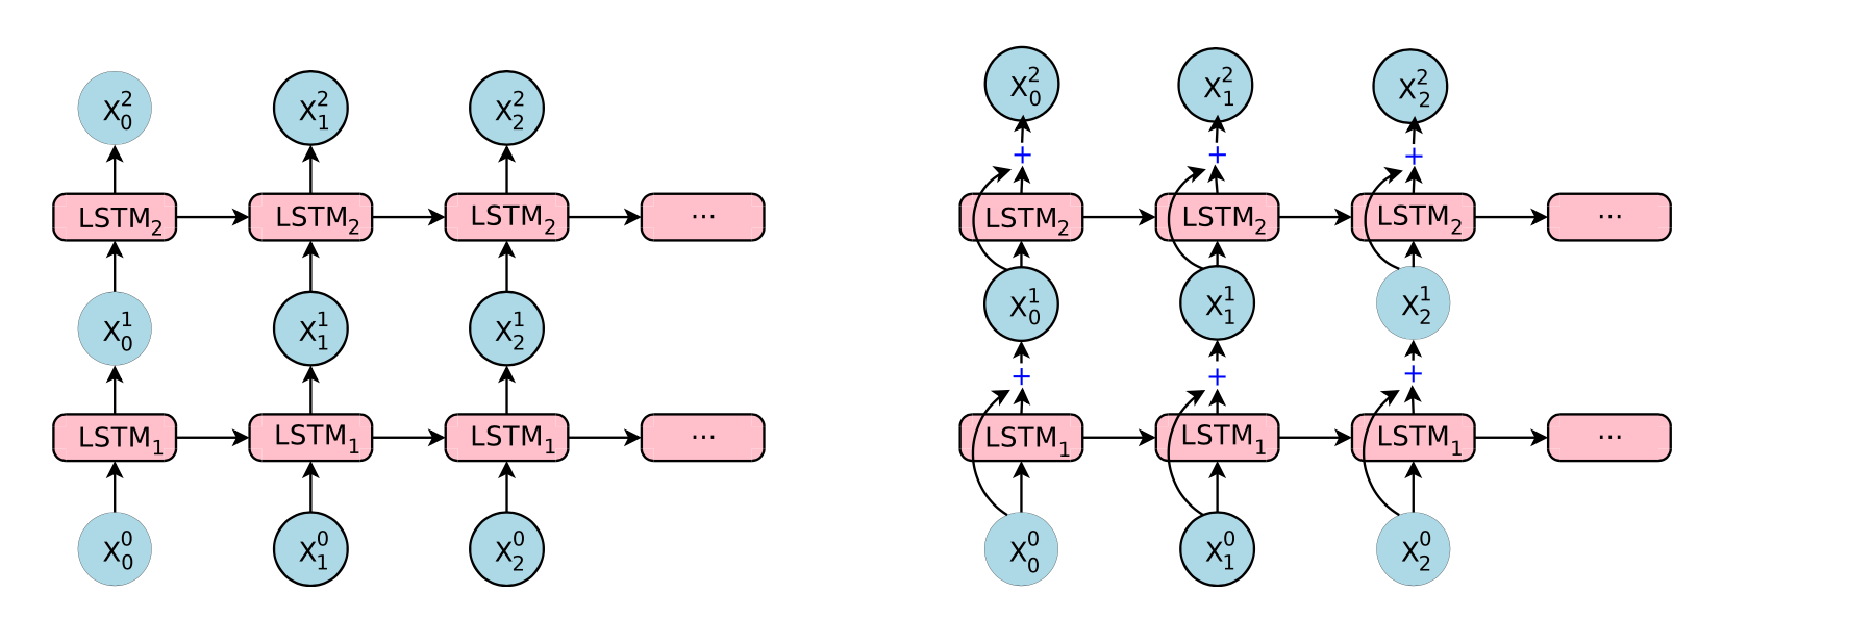
\includegraphics[width=1.\textwidth]{figures/lstm_layers.eps}
  \end{center}
  (The architecture on the right uses skip connections.)
\end{slide}

\begin{slide}{Performance}
  Before the appearance of transformers, LSTM-based language models performed
  consistently better than other architectures, and they are pretty competitive
  even now.\bigskip

  On 5 of the 9 language modeling datasets tracked by
  \href{http://http://nlpprogress.com}{NLP-progress}, models based on an
  LSTM-variant, the so-called Mogrifier LSTM have the best performance, and
  LSTM-based models are very close to the (transformer produced)
  state-of-the-art on 3 of the 4 remaining datasets.
\end{slide}

\section{References}

\begin{slide}{References}
  \bibliographystyle{plainnat}
  \begin{footnotesize}
    \bibliography{nlp_course.bib}    
  \end{footnotesize}
\end{slide}
\end{document}



%%% Local Variables:
%%% mode: latex 
%%% TeX-master: t
%%% End:

% LocalWords:  Tokenization Discriminative discriminative
